\section{Performance Analysis}
This section presents a comprehensive evaluation of our DSP framework across multiple dimensions. We first examine the online warmup behavior and predictor convergence patterns, demonstrating how the system adapts from a cold start to stable performance. We then compare our TD-learning approach against supervised learning alternatives and non-contextual heuristics, showing the advantages of our context-aware formulation. Finally, we provide a detailed cost breakdown analysis to illustrate how DSP achieves superior efficiency-cost tradeoffs compared to fixed-depth speculation strategies.

\subsection{Online Warmup}
In our experiment, we begin with a randomly initialized DistilBERT model at the initial stage of every setting and its predictions are naturally zero at the start. This results in the entire pipeline executing the target agent in a sequential manner during warm-up tasks without any additional cost increase. To expedite the reduction of warmup time, we start collecting training episodes online as the pipeline runs. Once enough episodes are gathered to meet the predefined batch size, the model undergoes its first training update. 

Our analysis across different settings reveals that the warmup duration varies depending on the API backbone. As shown in \cref{tab:warmup}, when using GPT-4.1-mini, it typically requires around \textbf{3–5 tasks} to warm up, as GPT-4.1-mini tends to generate longer sequences to complete each task. It enables faster collection of a sufficient number of training episodes. In contrast, when using DeepSeek-series models, the warmup phase is slower, requiring approximately \textbf{8–10 tasks} to collect enough training data. This discrepancy highlights the differences in the response times of different APIs and the resulting impact on the warmup efficiency.

\begin{table}[t]
\centering
\caption{Warm-up Phase Accuracy (First 13 Tasks)}
\label{tab:warmup}
\subcaption{OpenAGI}
\resizebox{\linewidth}{!}{

\begin{tabular}{l c c c c c c c c c c c c c}

\toprule
\textbf{Config} & Task 1 & Task 2 & Task 3 & Task 4 & Task 5 & Task 6 & Task 7 & Task 8 & Task 9 & Task 10 & Task 11 & Task 12 & Task 13 \\
\midrule
Direct-ReAct (GPT-4.1-mini) & 0 & 0.42 & 0.67 & 0.67 & 1 & 0.75 & 0.6 & 1 & 1 & 1 & 0.8 & 0.5 & 0.83 \\
Direct-ReAct (DeepSeek)     & 0 & 0 & 0 & 0 & 0 & 0.33 & 0.67 & 0 & 0.5 & 0.33 & 0.67 & 0.5 & 0.67 \\
CoT-MAD (GPT-4.1-mini)      & 0 & 0 & 0.5 & 0.5 & 0.67 & 0.25 & 0.38 & 0.75 & 0.5 & 0.8 & 0.57 & 0.6 & 0.8 \\
CoT-MAD (DeepSeek)          & 0 & 0 & 0 & 0 & 0 & 0 & 0 & 0 & 0.33 & 0.33 & 0.25 & 0.33 & 1 \\
\bottomrule
\end{tabular}
}
\subcaption{TravelPlanner}

\resizebox{\linewidth}{!}{

\begin{tabular}{l c c c c c c c c c c c c c}
\toprule
\textbf{Config} & Task 1 & Task 2 & Task 3 & Task 4 & Task 5 & Task 6 & Task 7 & Task 8 & Task 9 & Task 10 & Task 11 & Task 12 & Task 13 \\
\midrule
Direct-ReAct (GPT-4.1-mini) & 0 & 0 & 0.4 & 0.38 & 0.44 & 0.88 & 1 & 0.57 & 0.75 & 0.62 & 0.67 & 0.57 & 0.86 \\
CoT-MAD (GPT-4.1-mini)      & 0 & 0 & 0.62 & 1 & 0.29 & 1 & 0.43 & 0.83 & 0.57 & 0.71 & 0.71 & 1 & 0.57 \\
\bottomrule
\end{tabular}
}
\vspace{1em}
\end{table}

\subsection{Predictor Accuracy over Online Training}
To assess the effectiveness and stability of our online learning procedure, we examine predictor accuracy on the OpenAGI benchmark across sequential task segments. \cref{tab:predictor_accuracy} summarizes the mean and standard deviation of accuracy within non-overlapping 50-task windows, and \cref{fig:acc_trend} visualizes the global trend with a smoothed trajectory.

In the early stage (tasks 1–100), the predictor exhibits moderate accuracy and relatively high variance, reflecting the initial adaptation to unseen task distributions. As training progresses, accuracy consistently improves across all settings, accompanied by a steady reduction in variance. By the later segments (tasks 200–300), the predictor achieves substantially higher mean accuracy (0.70–0.76) while maintaining much lower variance, indicating convergence and stability.

These results demonstrate that online updates reliably enhance the predictor’s generalization ability to unseen tasks. Importantly, we observe no evidence of performance drift or instability in later stages. Instead, the predictor becomes increasingly accurate and stable, ensuring dependable speculative planning across diverse benchmarks.

\begin{table}[t]
\centering
\caption{Predictor Accuracy per 50-Task Segment on the OpenAGI benchmark (Mean $\pm$ SD)}
\label{tab:predictor_accuracy}
\resizebox{\linewidth}{!}{
\begin{tabular}{lcccc}
\toprule
\textbf{Task} & \textbf{Direct-ReAct (GPT)} & \textbf{Direct-ReAct (DeepSeek)} & \textbf{CoT-MAD (GPT)} & \textbf{CoT-MAD (DeepSeek)} \\
\midrule
1--50   & 0.600$\pm$0.351 & 0.465$\pm$0.317 & 0.641$\pm$0.342 & 0.459$\pm$0.334 \\
51--100 & 0.477$\pm$0.363 & 0.499$\pm$0.331 & 0.693$\pm$0.349 & 0.501$\pm$0.346 \\
101--150 & 0.689$\pm$0.256 & 0.701$\pm$0.352 & 0.675$\pm$0.285 & 0.564$\pm$0.334 \\
151--200 & 0.693$\pm$0.189 & 0.593$\pm$0.326 & 0.575$\pm$0.217 & 0.570$\pm$0.329 \\
201--250 & 0.755$\pm$0.207 & 0.657$\pm$0.280 & 0.621$\pm$0.198 & \textbf{0.704$\pm$0.239} \\
251--300 & 0.724$\pm$0.169 & \textbf{0.762$\pm$0.207} & 0.693$\pm$0.135 & 0.674$\pm$0.237 \\
301--312 & \textbf{0.761$\pm$0.205} & 0.707$\pm$0.201 & \textbf{0.760$\pm$0.130} & 0.698$\pm$0.259 \\
\bottomrule
\end{tabular}
}
\end{table}


\begin{figure}
\centering
    \begin{subfigure}[b]{0.44\textwidth}
        \centering
        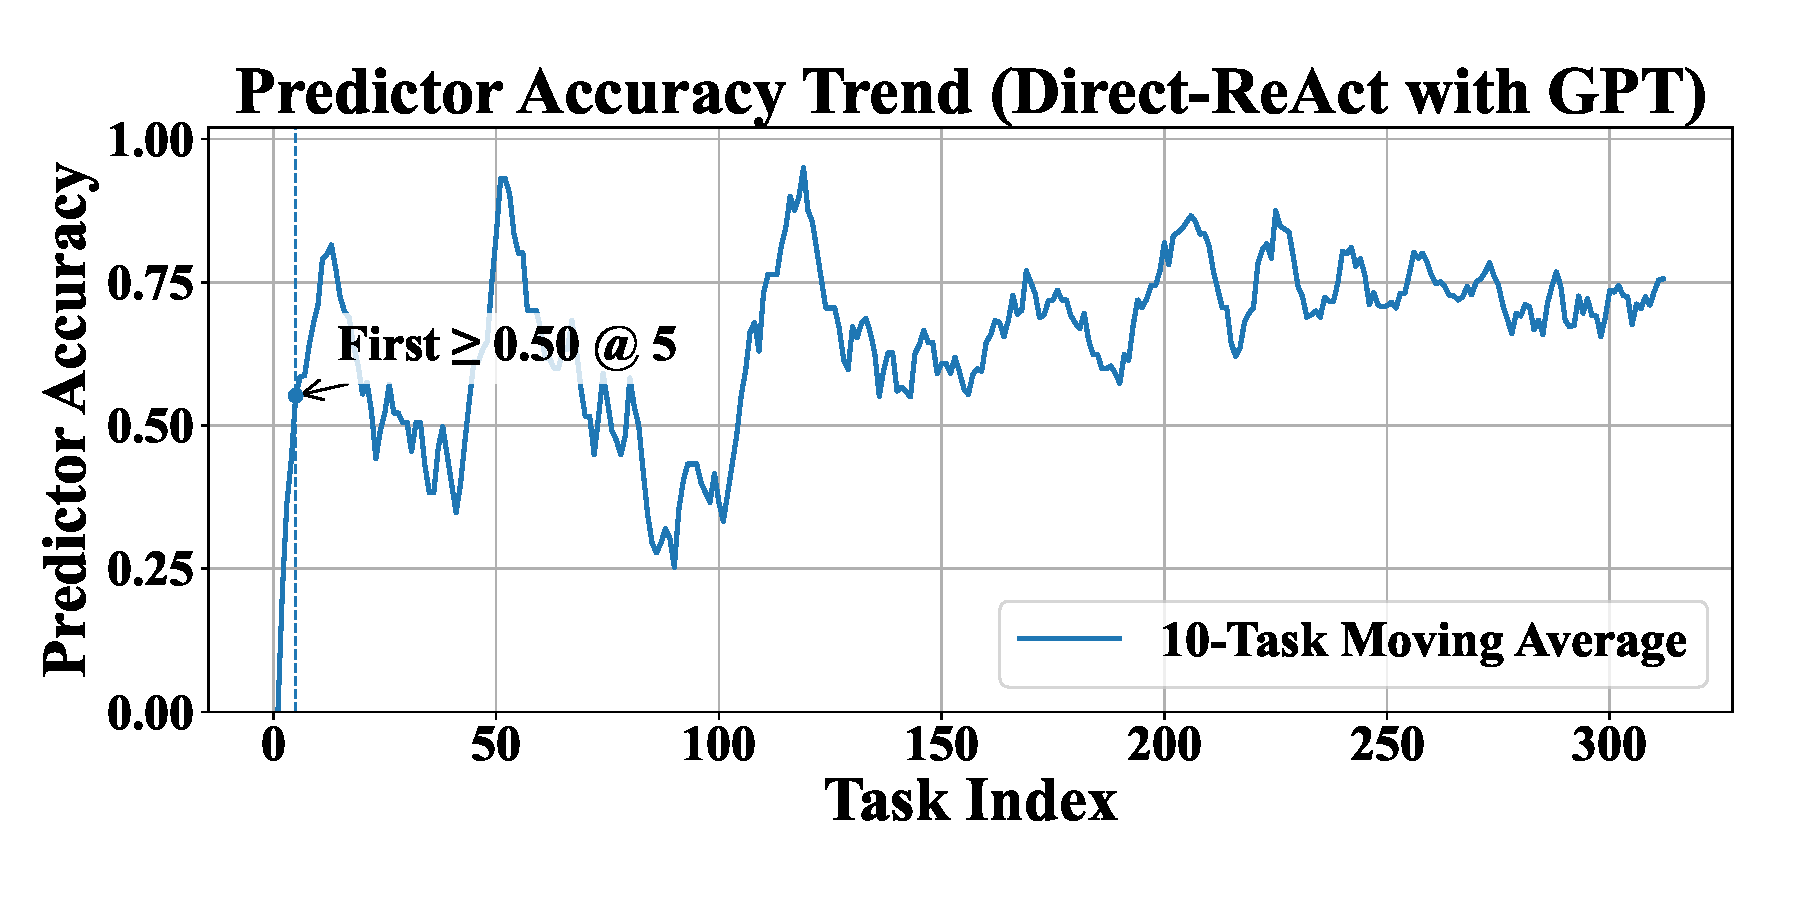
\includegraphics[width=\linewidth]{fig/direct_react_gpt_acc_trend.pdf}
        \captionsetup{skip=1pt}
        \caption{Direct-ReAct (GPT-4.1-mini)}
    \end{subfigure}
    \hfil
    \begin{subfigure}[b]{0.44\textwidth}
        \centering
        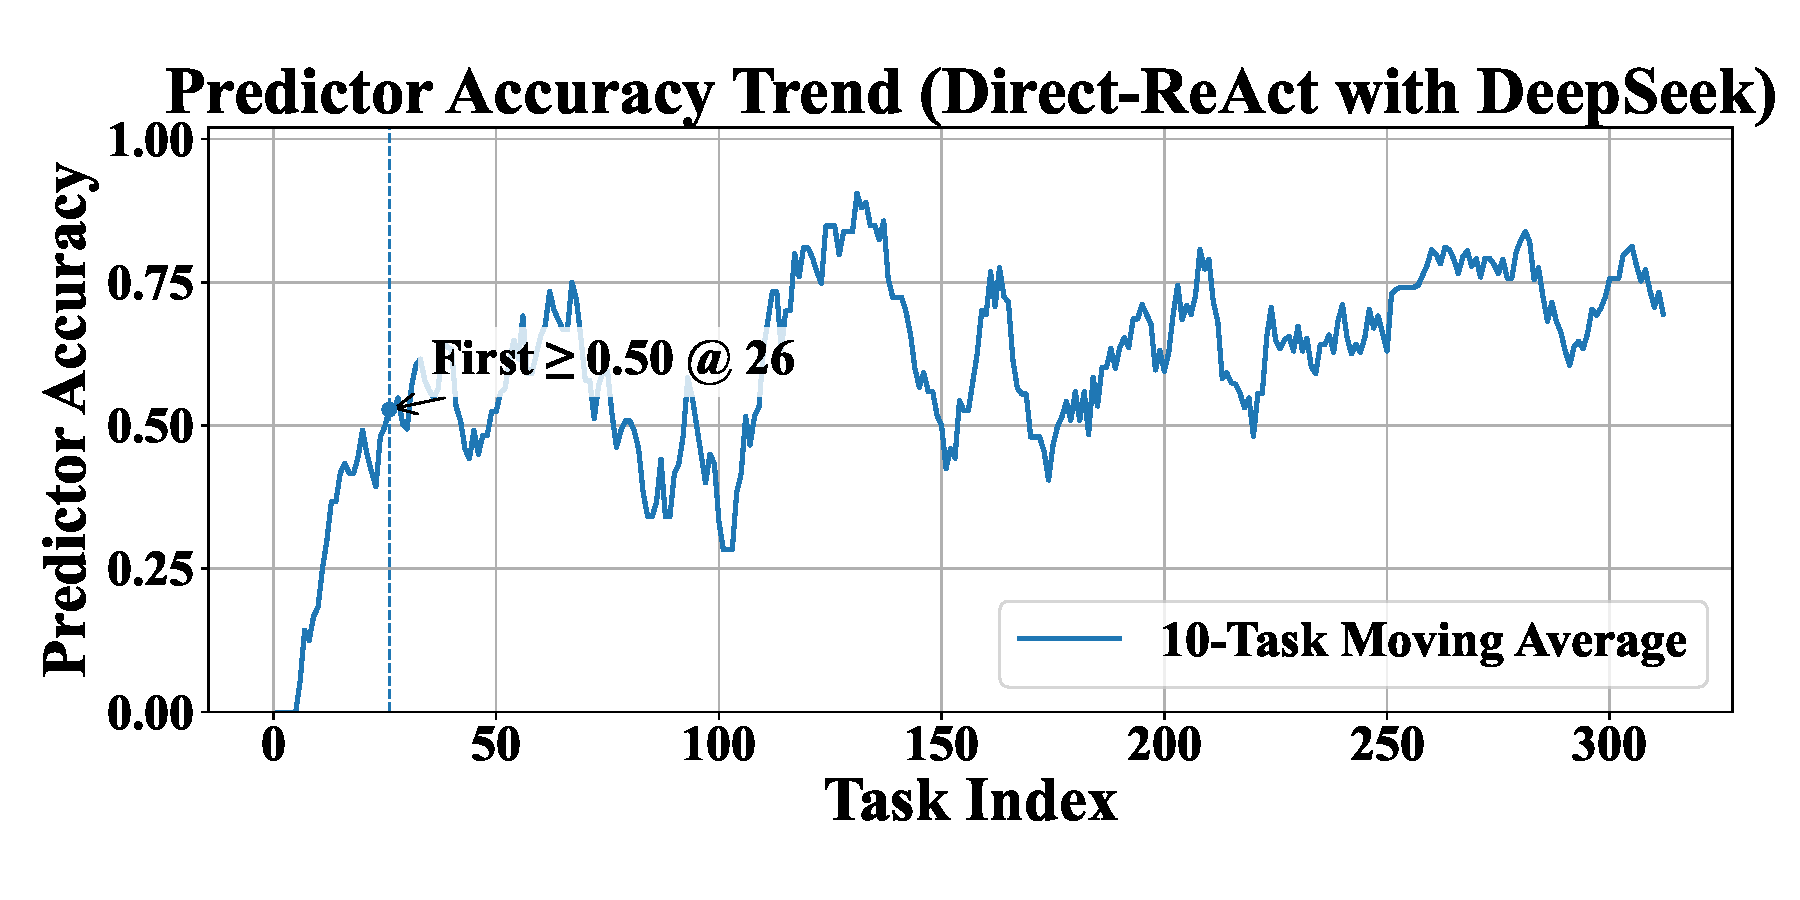
\includegraphics[width=\linewidth]{fig/direct_react_dpsk_acc_trend.pdf}
        \captionsetup{skip=1pt}
        \caption{Direct-ReAct (DeepSeek)}
    \end{subfigure}
    \vspace{0.5em}
    \begin{subfigure}[b]{0.44\textwidth}
        \centering
        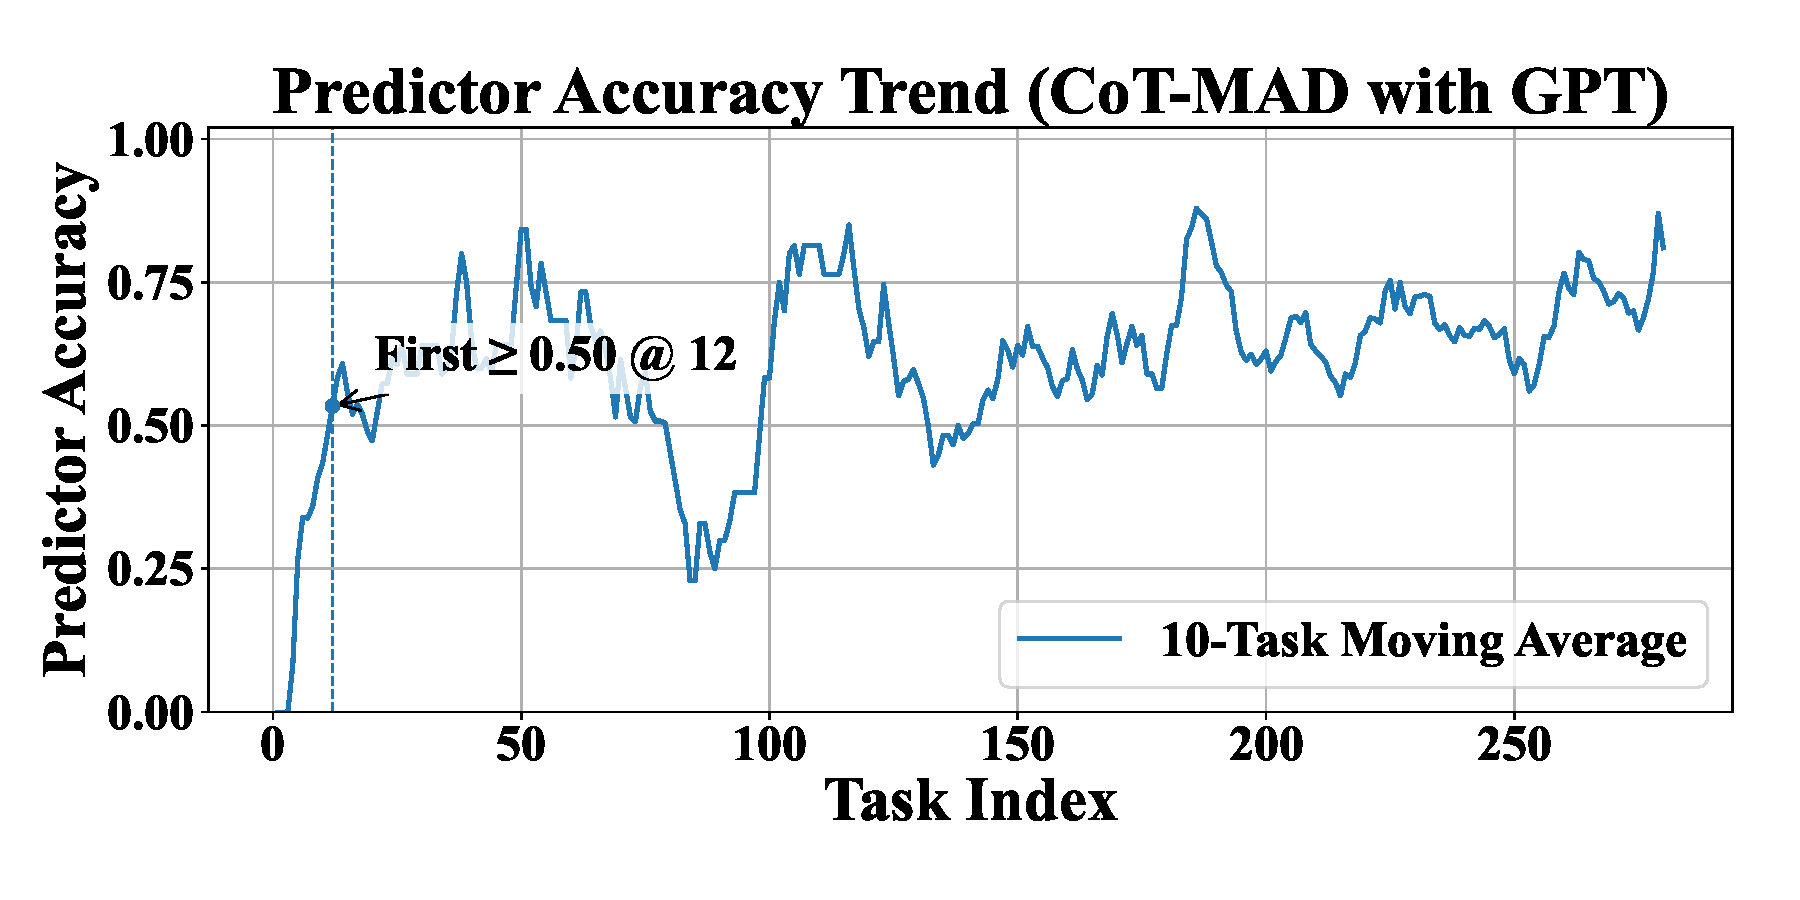
\includegraphics[width=\linewidth]{fig/cot_multi_agent_gpt_acc_trend.pdf}
        \captionsetup{skip=1pt}
        \caption{CoT-MAD (GPT-4.1-mini)}
    \end{subfigure}
    \hfil
    \begin{subfigure}[b]{0.44\textwidth}
        \centering
        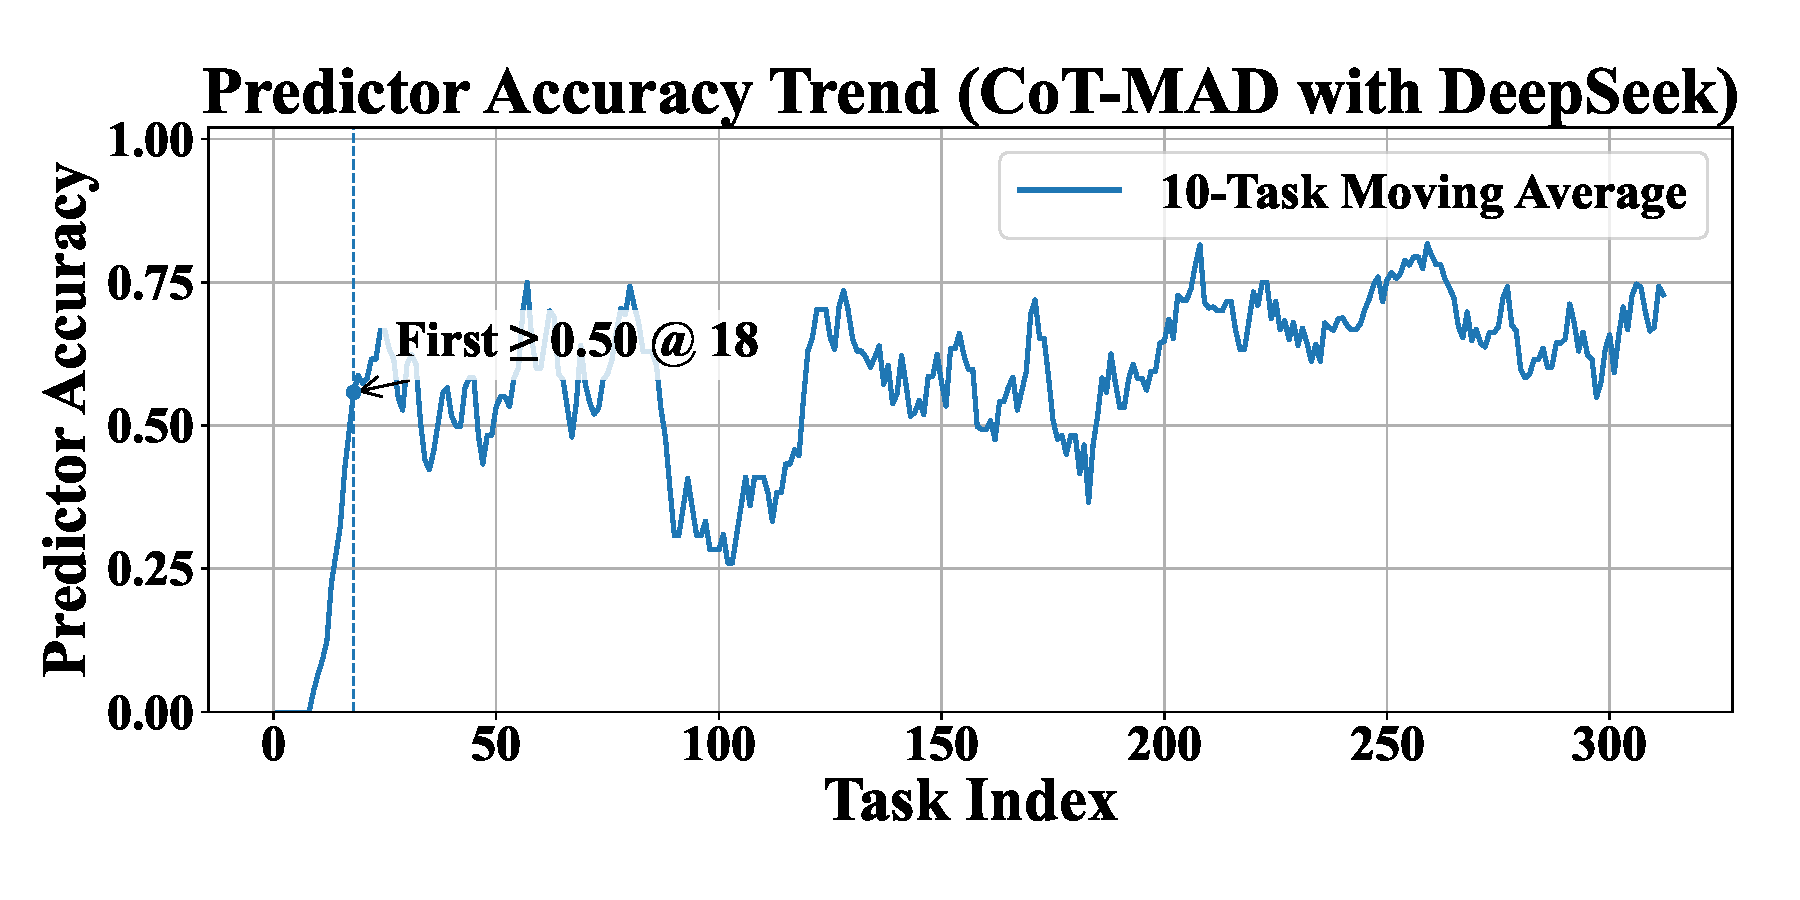
\includegraphics[width=\linewidth]{fig/cot_multi_agent_dpsk_acc_trend.pdf}
        \captionsetup{skip=1pt}
        \caption{CoT-MAD (DeepSeek)}
    \end{subfigure}
\captionsetup{skip=-1pt}
\caption{Predictor accuracy trends over online training across different settings. In all cases (Direct-ReAct and CoT-MAD with GPT-4.1-mini or DeepSeek), the predictor exhibits a clear upward trajectory in accuracy alongside decreasing variance, indicating improved generalization to unseen tasks and stable convergence without late-stage drift.}
\label{fig:acc_trend}
\end{figure}

\subsection{Supervised vs. Reinforcement Learning for Speculative Step Prediction}
We investigate two alternative formulations for speculative step prediction: supervised learning (SFT) and reinforcement learning (RL) with TD-based updates. While both are supported within our framework, we ultimately adopt the RL formulation for two key reasons.

Theoretically, supervised learning arises as a special case of our framework. When $\lambda=1$ and $\gamma=1$, the TD target reduces to the rollout length $G_t=k$, thus TD-learning reduces to online supervised learning. Additionally, $\lambda$-returns provide a tunable bias–variance tradeoff between Monte Carlo and bootstrapped estimates, offering greater flexibility than pure regression. Overall, our learning framework is a more generalized framework.

Emprically, training with fully supervised targets (i.e., $\lambda = 1, \gamma = 1$) produced overly conservative predictors. As shown in Table~\ref{tab:sft_vs_rl}, while the Dyn. (SFT) model achieves similar or even lower token cost savings as our TD-trained variant (Dyn. ($\tau$=0.5)), it consistently underperforms in terms of latency reduction. In most cases, the performance was even slower than a fixed $k = 2$ baseline, which is the minimal non‑trivial setting. Additionally, the Dyn. (SFT) model achieves lower accuracy across all settings compared to Dyn. ($\tau$=0.5) The experimental findings reveal the limitations of the supervised learning approach in this context. We attribute this to high variance in rollout-derived $k$ labels and the averaging tendency of regression, which causes SFT models to underestimate $k$ in uncertain regions.

\begin{table}[hbtp]
    \caption{Performance comparison of SFT vs. RL strategies on the \textbf{OpenAGI} benchmark.}
    \label{tab:sft_vs_rl}
    \centering
    \resizebox{\textwidth}{!}{
    \begin{tabular}{l l r r r r r r r r}
        \toprule
        \multirow{2}{*}{\bf Backbone} & \multirow{2}{*}{\bf Mode} 
            & \multicolumn{4}{c}{\bf Direct-ReAct} 
            & \multicolumn{4}{c}{\bf CoT-MAD} \\
        \cmidrule(lr){3-6} \cmidrule(lr){7-10}
            &   & T($\times$) & P($\times$) & G($\times$) & Cost($\times$) 
                & T($\times$) & P($\times$) & G($\times$) & Cost($\times$) \\
        \midrule
        \multirow{3}{*}{GPT-4.1-mini} 
            & Fix ($k$=2)        & 1.00 & 1.00 & 1.00 & 1.00  & 1.00 & 1.00 & 1.00 & 1.00 \\
            & Dyn. ($\tau$=0.5)  & 1.01 & 0.87 & 0.91 & \textbf{0.88}  & 0.98 & 0.95 & 0.95 & \textbf{0.95} \\
            & Dyn. (SFT)         & 1.05 & 0.86 & 0.91 & \textbf{0.88}  & 1.02 & 0.96 & 0.96 & 0.96 \\
        \midrule
        \multirow{3}{*}{DeepSeek} 
            & Fix ($k$=2)        & 1.00 & 1.00 & 1.00 & 1.00  & 1.00 & 1.00 & 1.00 & 1.00 \\
            & Dyn. ($\tau$=0.5)  & 1.04 & 0.93 & 0.94 & \textbf{0.93}  & 1.07 & 0.94 & 0.94 & \textbf{0.94} \\
            & Dyn. (SFT)         & 1.09 & 0.96 & 0.95 & 0.96  & 1.11 & 1.01 & 1.00 & 1.00 \\
        \bottomrule
    \end{tabular}
    }
\end{table}




\subsection{Evaluation on Non-Contextual Dynamic Heuristics}
To further demonstrate the advantage of our \textbf{Dynamic Speculative Planning (DSP)}, we implemented a non-contextual reward-driven black-box optimization heuristic using Bayesian Optimization (BO). 
Unlike DSP, this method does not exploit contextual state features, but instead attempts to learn a mapping from past speculative outcomes to effective $k$-values. 
Specifically, BO maintains a surrogate model (Random Forest Regressor) to predict the expected reward for different $k$-values based on past selection outcomes. 
The reward is defined as:
\[
R(k) = \frac{1}{|k - k^{\ast}| + 1},
\]
where $k^{\ast}$ denotes the ground-truth speculative depth. 
This formulation incentivizes the selection of $k$ values closer to the true horizon. 
For the exploration–exploitation tradeoff, we adopted a lightweight $\epsilon$-Greedy acquisition strategy ($\epsilon=0.1$), 
which maintains efficiency during online updates. 

As shown in Table~\ref{tab:bo_results}, in Direct-ReAct setting with GPT backbone, BO achieves performance comparable to the fixed $k=2$ baseline, but fails to realize the dynamic acceleration potential of DSP. Compared to our DSP variant with $\tau=0.5$, BO yields a similar latency reduction yet incurs \textbf{10\% higher total cost}. Conversely, when compared with DSP at $\tau=0.8$, BO matches token cost but delivers \textbf{significantly less acceleration}. 
Direct-ReAct setting with DeepSeek backbone and CoT-MAD setting with GPT backbone only contains first 250 tasks. In these two settings, BO consistently lags behind DSP variants as it delivers substantially worse acceleration.

These results highlight that DSP maintains a superior Pareto frontier, achieving a more favorable balance between efficiency and resource usage through context-aware prediction. 

\begin{table*}[t]
\centering
\caption{Performance Comparison between Bayesian Optimization and DSP on OpenAGI (First 200 Tasks)}
\label{tab:bo_results}
\resizebox{\linewidth}{!}{
\begin{tabular}{lcccccccccccc}
\toprule
 & \multicolumn{4}{c}{Direct-ReAct (GPT-4.1-mini)} 
 & \multicolumn{4}{c}{Direct-ReAct (DeepSeek)} 
 & \multicolumn{4}{c}{CoT-MAD (GPT-4.1-mini)} \\
\cmidrule(lr){2-5} \cmidrule(lr){6-9} \cmidrule(lr){10-13}
\textbf{Method} 
 & Time & Prompt & Gen & Cost 
 & Time & Prompt & Gen & Cost
 & Time & Prompt & Gen & Cost \\
\midrule
\textbf{Fixed-k} & & & & & & & & & & & & \\
$k = 2$ & 1.00 & 1.00 & 1.00 & 1.00 & 1.00 & 1.00 & 1.00 & 1.00 & 1.00 & 1.00 & 1.00 & 1.00 \\
$k = 4$ & 0.90 & 1.47 & 1.21 & 1.35 & 0.85 & 1.49 & 1.44 & 1.46 & 0.81 & 1.35 & 1.34 & 1.32 \\
$k = 6$ & 0.88 & 2.00 & 1.47 & 1.74 & 0.84 & 1.85 & 1.76 & 1.82 & 0.77 & 1.69 & 1.63 & 1.62 \\
\midrule
\textbf{DSP} & & & & & & & & & & & & \\
$\tau=0.5$  & \textbf{0.99} & 0.94 & 0.96 & \textbf{0.94} & \textbf{1.02} & 0.95 & 0.96 & \textbf{0.96} & \textbf{0.92} & 1.03 & 1.02 & \textbf{1.03} \\
$\tau=0.8$  & 0.94 & 1.06 & 1.03 & 1.04 & 0.98 & 1.02 & 1.04 & 1.02 & 0.84 & 1.10 & 1.10 & 1.10 \\
$\tau=0.9$  & 0.93 & 1.14 & 1.06 & 1.10 & 0.92 & 1.09 & 1.08 & 1.09 & 0.82 & 1.15 & 1.14 & 1.14 \\
$\tau=0.95$ & 0.91 & 1.22 & 1.13 & 1.17 & 0.91 & 1.20 & 1.22 & 1.21 & 0.81 & 1.30 & 1.29 & 1.28 \\
$\tau=0.99$ & 0.90 & 1.37 & 1.21 & 1.29 & 0.87 & 1.42 & 1.41 & 1.41 & 0.81 & 1.39 & 1.37 & 1.36 \\
offset=1    & 0.91 & 1.15 & 1.08 & 1.11 & 0.93 & 1.12 & 1.14 & 1.13 & 0.84 & 1.15 & 1.13 & 1.13 \\
offset=2    & 0.90 & 1.35 & 1.17 & 1.27 & 0.85 & 1.30 & 1.31 & 1.30 & 0.76 & 1.33 & 1.30 & 1.30 \\
\midrule
\textbf{Heuristic} & & & & & & & & & & & & \\
BO & \textbf{1.03} & 0.98 & 0.98 & \textbf{0.97} & \textbf{1.09} & 0.98 & 0.94 & \textbf{0.95} & \textbf{1.10} & 1.03 & 0.95 & \textbf{1.00} \\
\bottomrule
\end{tabular}}
\end{table*}

\subsection{DSP Cost Broken-Down} 
The cost breakdown data for Fix and Dynamic Speculative Planning across different asymmetry parameters $\tau$ and different offset is presented in Table.\ref{tab:cost_broken_down_table}. In both DSP settings, the cost structure maintains the same general pattern observed in fixed-$k$ Speculative Planning, with the majority of tokens being consumed by target agent operations in input prompt; but $\tau$ parameter effectively controls the aggressiveness of speculation, showing clear patterns in cost reduction:

At the most conservative setting where $\tau$ = 0.5, the DSP reduces the average redundant token consumption from +10,748.3 to +672.2 in setting 1 and from +20,424.0 to +8,508.7 redundant tokens in setting 2, respectively, comparing with the most conservative fixed-$k$ setting where $k=2$. \textit{This represents an around 71\% reduction in redundant token consumption.} At the most aggressive setting where $\tau$ = 0.99, the DSP also reduces the average total token consumption from +52,664.6 to +14,452.6 in setting 1 and from +96,927.3 to +50,977.8 in setting 2, respectively, comparing with the most aggressive fixed-$k$ setting where $k=6$. \textit{This also represents an around 50\% reduction in redundant token consumption.} The graduated scaling of costs with the $\tau$ parameter provides practitioners with fine-grained control over the efficiency-cost balance, enabling precise system calibration that fixed-$k$ approaches cannot match.


\begin{table}[t]
\caption{Speculative Planning cost broken-down on \textbf{OpenAGI} benchmark with \textbf{GPT} backbone}
\label{tab:cost_broken_down_table}
\centering
\subcaptionbox{Direct-ReAct (Setting 1)\label{cost_broken_down_s1}}{
\resizebox{\textwidth}{!}{
\begin{tabular}{lrrrrrrr}
\toprule
Plan Type & Approx Prompt & Approx Generation & Target Prompt & Target Generation & Total Prompt & Total Generation & Total Token \\
\midrule

\midrule
Normal Plan & 6040.3 & 108.6 & 12715.6 & 1906.7 & 18755.9 & 2015.3 & 20771.2 \\
\hdashline
Fix (k=2) & 10759.8 & 165.7 & 18162.7 & 2431.2 & 28922.5 & 2596.9 & 31519.4 \\
Fix (k=4) & 19894.5 & 281.9 & 26610.1 & 2963.1 & 46504.6 & 3245.1 & 49749.7 \\
Fix (k=6) & 34124.0 & 369.2 & 35079.7 & 3862.9 & 69203.7 & 4232.1 & 73435.8 \\
\hdashline
Dyn. ($\tau$ = 0.5) & 6457.7 & 115.0 & 13022.8 & 1965.6 & 19480.5 & 2081.6 & 21443.4 \\
Dyn. ($\tau$ = 0.8) & 7454.8 & 130.9 & 14348.4 & 1994.6 & 21803.1 & 2125.5 & 23928.6 \\
Dyn. ($\tau$ = 0.9) & 8745.6 & 148.9 & 16062.6 & 2185.7 & 24808.2 & 2334.6 & 27142.8 \\
Dyn. ($\tau$ = 0.95) & 9226.2 & 154.7 & 16407.2 & 2176.9 & 25633.4 & 2331.6 & 27965.0 \\
Dyn. ($\tau$ = 0.99) & 12307.0 & 195.1 & 20140.0 & 2581.7 & 32447.0 & 2776.8 & 35223.8 \\
\hdashline
Dyn. (offset = 1) & 9576.3 & 163.9 & 17381.4 & 2293.0 & 26957.7 & 2456.9 & 29414.7 \\
Dyn. (offset = 2) & 12999.8 & 206.1 & 20254.3 & 2457.7 & 33254.1 & 2663.8 & 35917.9 \\
\midrule
\textbf{Redundant Cost} & & & & & & &\\
\midrule
$\Delta$ Fix (k = 2) & +4719.5 & +57.1 & +5447.1 & +524.5 & +10166.6 & +581.6 & +10748.3 \\
$\Delta$ Fix (k = 4) & +13854.2 & +173.3 & +13894.4 & +1056.5 & +27748.7 & +1229.8 & +28978.5 \\
$\Delta$ Fix (k = 6) & +28083.7 & +260.6 & +22364.1 & +1956.2 & +50447.8 & +2216.8 & +52664.6 \\
\hdashline
\textbf{$\Delta$ Dyn. ($\tau$ = 0.5)} & +417.4 & +6.4 & +307.2 & +58.9 & \textbf{+724.6} & \textbf{+66.3} & \textbf{+672.2} \\
$\Delta$ Dyn. ($\tau$ = 0.8) & +1414.5 & +22.3 & +1632.8 & +87.9 & +3047.2 & +110.2 & +3157.4 \\
$\Delta$ Dyn. ($\tau$ = 0.9) & +2705.3 & +40.3 & +3347.0 & +279.0 & +6052.3 & +319.3 & +6371.6 \\
$\Delta$ Dyn. ($\tau$ = 0.95) & +3185.9 & +46.1 & +3691.6 & +270.2 & +6877.5 & +316.3 & +7193.8 \\
$\Delta$ Dyn. ($\tau$ = 0.99) & +6266.7 & +86.5 & +7424.4 & +675.0 & +13691.1 & +761.5 & +14452.6 \\
\hdashline
$\Delta$ Dyn. (offset = 1) & +3536.0 & +55.3 & +4665.8 & +386.3 & +8201.8 & +441.6 & +8643.5 \\
$\Delta$ Dyn. (offset = 2) & +6959.5 & +97.5 & +7538.7 & +551.0 & +14498.2 & +648.5 & +15146.7 \\
\bottomrule
\end{tabular}
}
}
\subcaptionbox{CoT-MAD (Setting 2)\label{cost_broken_down_s2}}{
\resizebox{\textwidth}{!}{
\begin{tabular}{lrrrrrrr}
\toprule
Plan Type & Approx Prompt & Approx Generation & Target Prompt & Target Generation & Total Prompt & Total Generation & Total Token \\
\midrule
Normal Plan & 5422.5 & 1701.3 & 35968.4 & 7332.8 & 41390.9 & 9034.0 & 50424.9 \\
\hdashline
Fix (k=2) & 8158.9 & 2435.4 & 50373.5 & 9881.1 & 58532.4 & 12316.5 & 70848.9 \\
Fix (k=4) & 13799.2 & 3884.8 & 70283.3 & 13253.9 & 84082.5 & 17138.7 & 101221.2 \\
Fix (k=6) & 26065.3 & 5466.1 & 97668.0 & 18152.8 & 123733.3 & 23618.9 & 147352.2 \\
\hdashline
Dyn. ($\tau$ = 0.5) & 6429.6 & 1946.9 & 42200.3 & 8356.7 & 48629.9 & 10303.7 & 58933.6 \\
Dyn. ($\tau$ = 0.8) & 7671.9 & 2330.3 & 48703.2 & 9577.7 & 56375.1 & 11908.0 & 68283.1 \\
Dyn. ($\tau$ = 0.9) & 8682.5 & 2590.9 & 52586.8 & 10255.2 & 61269.3 & 12846.1 & 74115.5 \\
Dyn. ($\tau$ = 0.95) & 10417.5 & 3043.1 & 58605.2 & 11353.2 & 69022.7 & 14396.4 & 83419.1 \\
Dyn. ($\tau$ = 0.99) & 13857.5 & 3848.7 & 70281.1 & 13415.5 & 84138.5 & 17264.2 & 101402.7 \\
\hdashline
Dyn. (offset = 1) & 8978.2 & 2699.9 & 54749.3 & 10715.0 & 63727.4 & 13414.9 & 77142.3 \\
Dyn. (offset = 2) & 11256.8 & 3276.3 & 61864.3 & 11828.1 & 73121.1 & 15104.4 & 88225.6 \\
\midrule
\textbf{Redundant Cost} & & & & & & &\\
\midrule
$\Delta$ Fix (k = 2) & +2736.4 & +734.1 & +14405.1 & +2548.3 & +17141.5 & +3282.4 & +20424.0 \\
$\Delta$ Fix (k = 4) & +8376.7 & +2183.5 & +34314.9 & +5921.2 & +42691.6 & +8104.7 & +50796.3 \\
$\Delta$ Fix (k = 6) & +20642.8 & +3764.9 & +61699.6 & +10820.0 & +82342.4 & +14584.9 & +96927.3 \\
\hdashline
\textbf{$\Delta$ Dyn. ($\tau$ = 0.5)} & +1007.1 & +245.6 & +6231.9 & +1023.9 & \textbf{+7239.0} & \textbf{+1269.7} & \textbf{+8508.7} \\
$\Delta$ Dyn. ($\tau$ = 0.8) & +2249.4 & +629.0 & +12734.8 & +2244.9 & +14984.2 & +2874.0 & +17858.2 \\
$\Delta$ Dyn. ($\tau$ = 0.9) & +3260.0 & +889.6 & +16618.4 & +2922.4 & +19878.4 & +3812.1 & +23690.6 \\
$\Delta$ Dyn. ($\tau$ = 0.95) & +4995.0 & +1341.8 & +22636.8 & +4020.4 & +27631.8 & +5362.4 & +32994.2 \\
$\Delta$ Dyn. ($\tau$ = 0.99) & +8435.0 & +2147.4 & +34312.7 & +6082.7 & +42747.6 & +8230.2 & +50977.8 \\
\hdashline
$\Delta$ Dyn. (offset = 1) & +3555.7 & +998.6 & +18780.9 & +3382.2 & +22336.5 & +4380.9 & +26717.4 \\
$\Delta$ Dyn. (offset = 2) & +5834.3 & +1575.0 & +25895.9 & +4495.3 & +31730.2 & +6070.4 & +37800.7 \\
\bottomrule
\end{tabular}
}
}
\end{table}
